\documentclass[a4paper,12pt]{article}

\usepackage[utf8]{inputenc}
\usepackage[T1]{fontenc}
\usepackage{color}
\definecolor{grey}{rgb}{0.9,0.9,0.9}
\definecolor{teal}{rgb}{0.0,0.5,0.5}
\definecolor{violet}{rgb}{0.5,0,0.5}
\usepackage[margin=2.5cm]{geometry}
\usepackage{graphicx}
\usepackage[francais]{babel}
\usepackage[babel=true]{csquotes}
\usepackage{listings}

\title{TP3 - Analyse de concepts}
\author{\textsc{Paul Chaignon} - \textsc{Ulysse Goarant}}
\date{\today}

\begin{document}
\lstset{language=Prolog, breaklines=true}

\maketitle

\section{Système solaire}
\subsection{Question 1}
Le treillis associé aux planètes est le suivant :
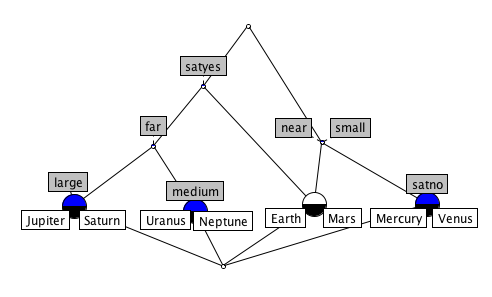
\includegraphics[width=400px]{question1.png}

\subsection{Question 2}
De part sa spécificité, un exemple tel que Pluton modifie fortement la structure du treillis. On en déduit que l'exception a autant d'importance que les règles.

\subsection{Question 3}
\textit{Show only exact matches} affiche uniquement le comptage des exemples qui possèdent les attributs en intention, alors que \textit{Show all matches} affiche le comptage des exemples possédant simplement et non nécessairement de manière exclusive l'attribut.

\section{Echelle conceptuelle}
\subsection{Question 4}
La taille des disques durs a une échelle et des attributs de type numérique. Les types de bus système ont une échelle et des attributs de type nominal. Les moyens de distribution ont une échelle de type nominal et des attributs de type booléen.

\section{Recensement américain : implications-règles d'association}
\subsection{Question 5}
On constate que la base d'implication est contenue dans les règles extraites.

\subsection{Question 6}
Il n'est bien sûr pas visuellement exploitable. % TODO: repondre suite question

\section{Base de comics gérée avec Camelis}
\subsection{Question 7}


\subsection{Question 8}
Le contexte contient 628 objets qui possèdent 6 attributs.

\subsection{Question 9}
En utilisant la navigation dans la propriété \textit{éditeur}, on trouve que le nombre de séries par éditeur varie de 11 à 72 selon ce dernier. Selon la même méthode appliquée à la propriété \textit{dessinateur}, on détermine que le dessinateur ayant le plus de comics est Corben (Richard).

\subsection{Question 12}
A l'aide de la requête \textit{not Genre ?}, on trouve que textit{Blondie} n'a pas de genre.

\end{document}